\documentclass[12pt,a4paper]{article}
\usepackage[a4paper]{geometry}
\usepackage{fullpage}
\usepackage{url}
\usepackage[backend=bibtex]{biblatex}
\usepackage{caption}
\usepackage[utf8]{inputenc}
\usepackage{enumerate}
\usepackage{tabularx}
\usepackage{graphicx}
\usepackage{float}
\usepackage{color}
\usepackage{amssymb,amsmath,wasysym}
\usepackage{enumitem}

\addbibresource{bib1.bib}

\begin{document}

\title{Computational Intelligence, SS2017, Assigment 3}

\author{%
\name{Lucas Reeh}
\email{lreeh@student.tugraz.at}
}
\date{\today}

\begin{titlepage}
   \begin{center}
     \begin{huge}
		   %% Update assignment number here
           \textbf{Assignment 4}
     \end{huge}
   \end{center}

   \begin{center}
     \begin{large}
           Computational Intelligence, SS2017
     \end{large}
   \end{center}

   \begin{center}
 \begin{tabularx}{\textwidth}{|>{\hsize=.33\hsize}X|>{\hsize=.33\hsize}X|>{\hsize=.33\hsize}X|} 

           \hline
           \multicolumn{3}{|c|}{\textbf{Team Members}} \\
           \hline
           Last name & First name & Matriculation Number \\
           \hline
           Reeh & Lucas & 00630128 \\
           \hline

     \end{tabularx}
   \end{center}
\end{titlepage}

\tableofcontents
\listoffigures

\newpage

\section{Expectation Maximization Algorithm}

\begin{figure}[H]
  \centering
  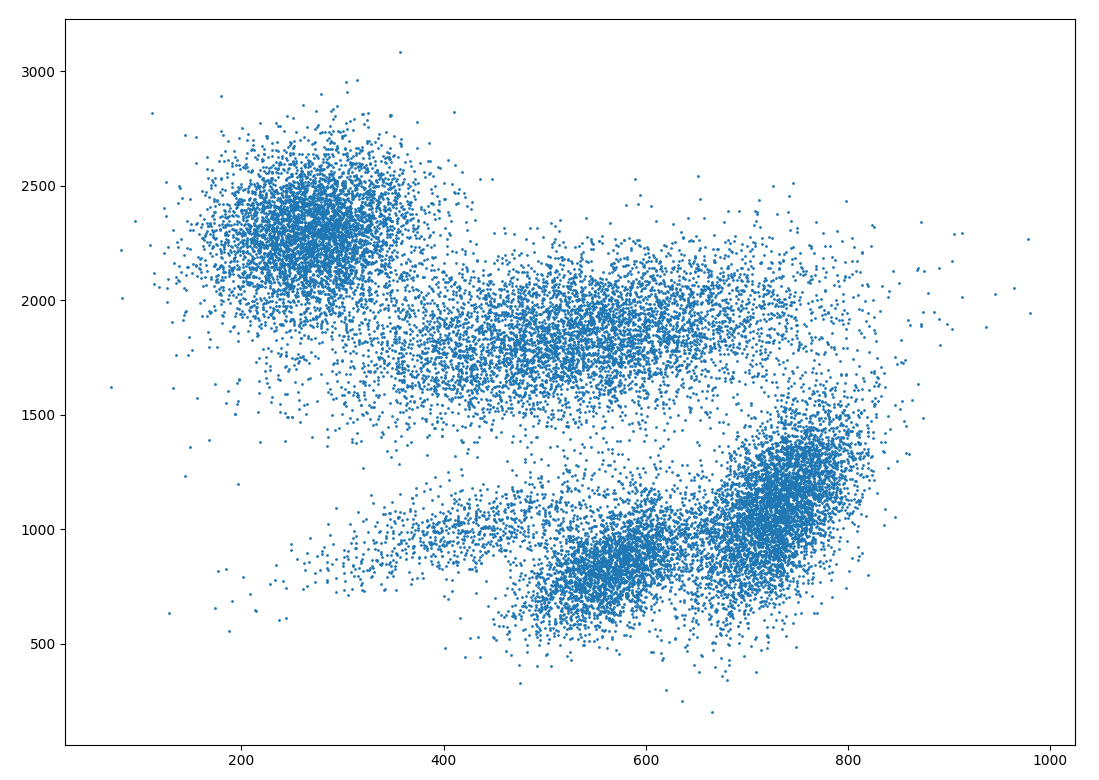
\includegraphics[width=0.8\textwidth]{figures/1_0.png}
	\caption{Training Data}
	\label{1_0}
\end{figure}

\setcounter{enumi}{2}
\begin{enumerate}[start=2,label*={\arabic*.}]
  % 1
  % 2
  \item Correct number of components $M = 5$ (fixed random seed)
  
\begin{figure}[H]
  \centering
  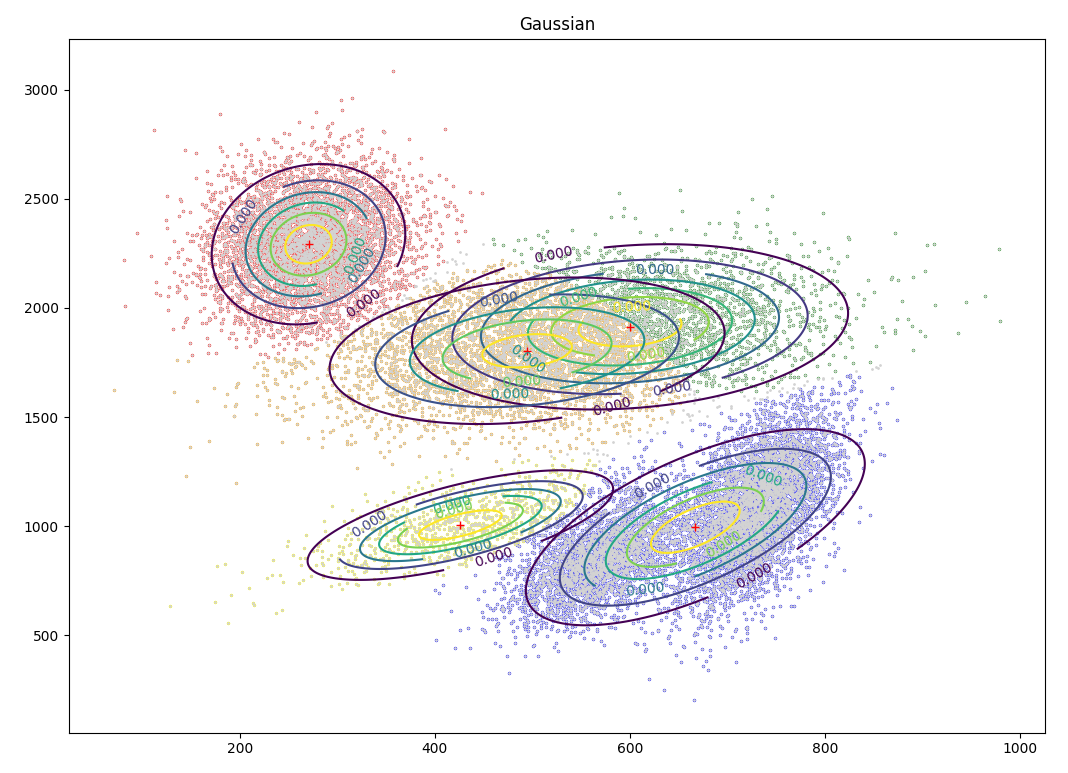
\includegraphics[width=0.8\textwidth]{figures/1_2.png}
	\caption{EM using $M = 5$}
	\label{1_2}
\end{figure}

Figure \ref{1_2_compare} shows test-data overlayed by gaussian countours from
EM-algorithm to compare to actual values.

\begin{figure}[H]
  \centering
  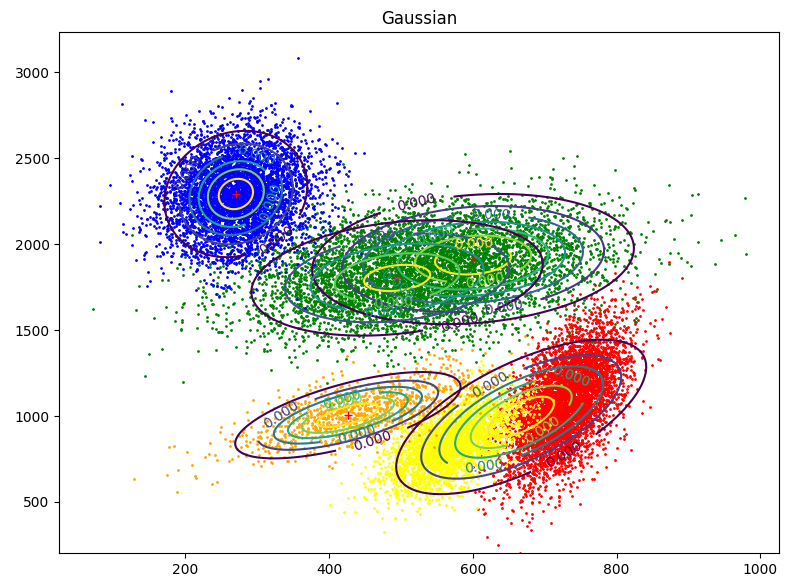
\includegraphics[width=0.8\textwidth]{figures/1_2_compare.png}
	\caption{EM compared to test data}
	\label{1_2_compare}
\end{figure}
  
  % 3
  \item Initialization was choosen like mentioned in lecture
  noted\autocite{lecuter_notes_spsc}. Wrong number of components can lead to
  unexpected results ranging from complete jibberish to good matching
  distributions.
  
  Other findings with different $\Theta$ values:
  \begin{itemize}
    \item Random seed can have great effect on the result, see Hint below.
    \item divergence when choosing wrong parameters (eg. wrong $\Sigma_0$)
    \item zero division when choosing $\alpha_0 = 0$.
    \item weird linalg errors (\texttt{numpy.linalg.linalg.LinAlgError}) when
    using identity matrix for $\Sigma_0$.
  \end{itemize}
  
  % 4
  \item Log-Likelihood function is converging very fast to the second iteration
  but slows down from there see Figure \ref{1_2_log}. Even logarithmic scaled
  y-axis on the plot had no improvement on the visualization.

\begin{figure}[H]
  \centering
  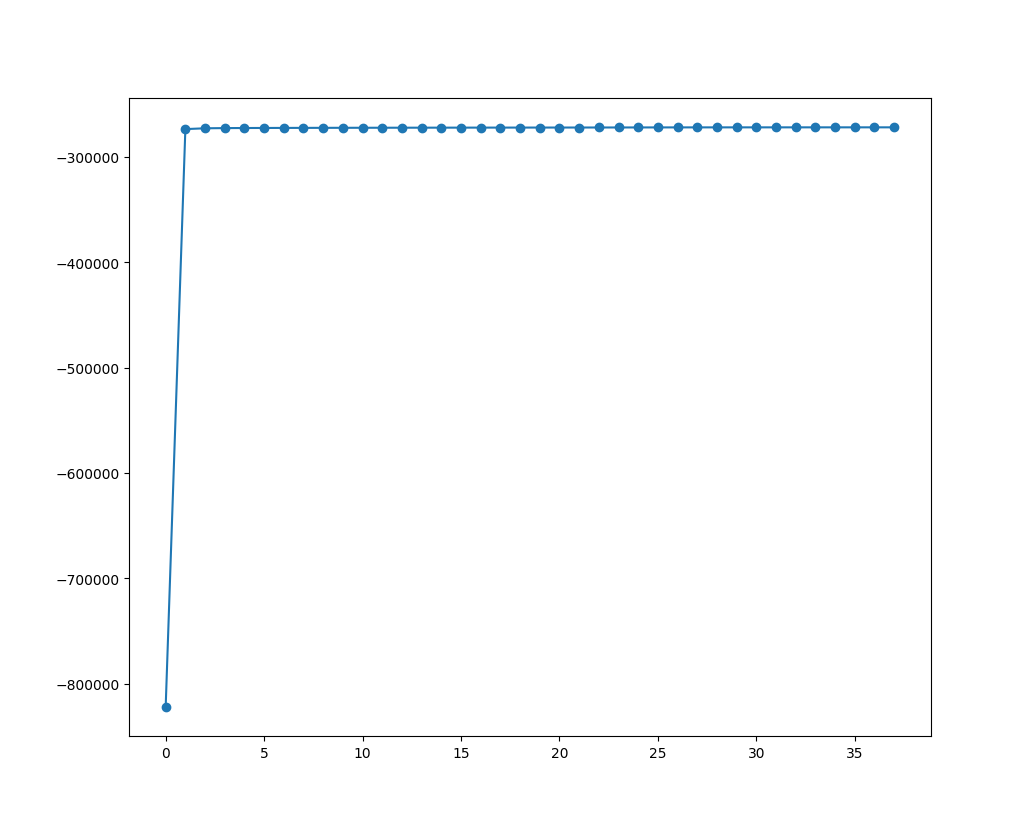
\includegraphics[width=0.8\textwidth]{figures/1_2_log.png}
	\caption{EM Log-Likelood progress over iterations}
	\label{1_2_log}
\end{figure}
  
  As you can see in Figure \ref{1_2_log_1} Skipping data from the first
  iteration gives a much clearer picture. Now convergence (slightly logarithmic)
  is recognizable.
  
\begin{figure}[H]
  \centering
  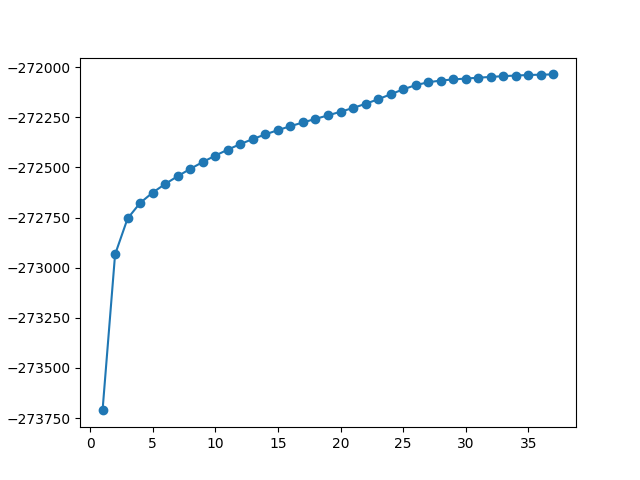
\includegraphics[width=0.8\textwidth]{figures/1_2_log_1.png}
	\caption{EM Log-Likelood progress over iterations (without the first)}
	\label{1_2_log_1}
\end{figure}
  
  % 5
  \item If $\Sigma$ is a diagonal matrix the distributions are not tilted and
  only expand along the axises (x, y). This sometimes leads to faster
  convergence but not so accurate matching.
  
\begin{figure}[H]
  \centering
  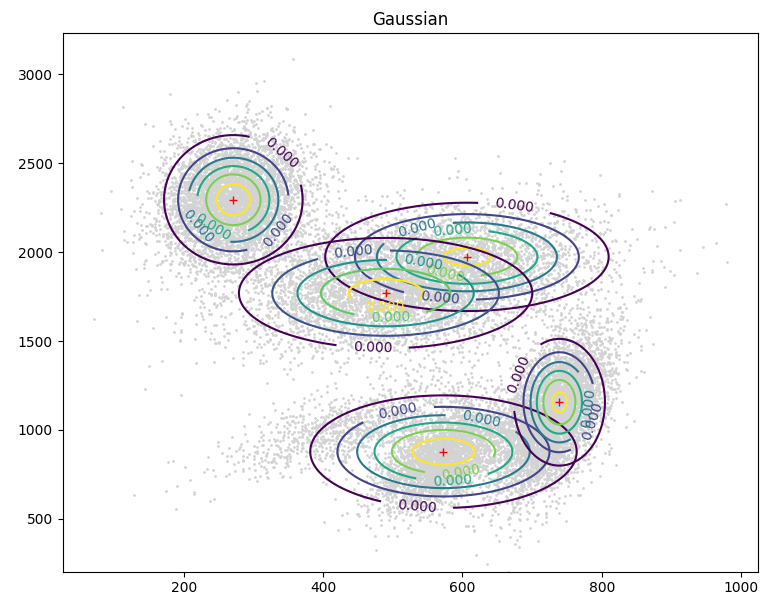
\includegraphics[width=0.8\textwidth]{figures/1_0_diag.png}
	\caption{Using diagonal matrix for $\Sigma$}
	\label{1_0_diag}
\end{figure}
  
\begin{figure}[H]
  \centering
  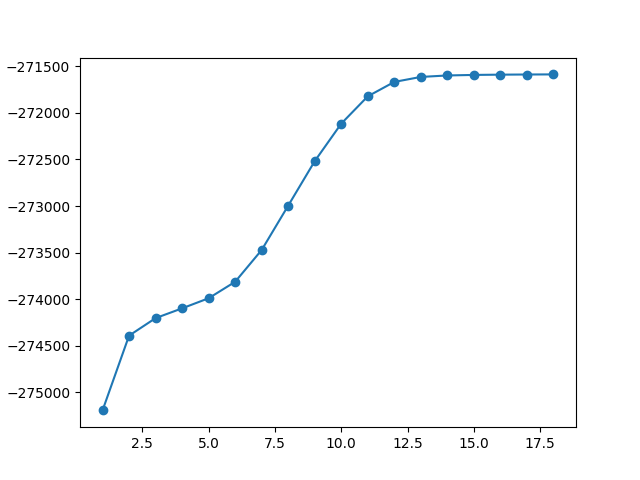
\includegraphics[width=0.8\textwidth]{figures/1_0_diag_log.png}
	\caption{EM Log-Likelood using diagonal matrix for $\Sigma$}
	\label{1_0_diag_log}
\end{figure}
  
  From time to time matrix computation errors occur within the
  given likelihood framework function: \texttt{ValueError: zero-size array to
  reduction operation minimum which has no identity} with no diagonal matrix, i
  guess rounding errors and zero values in the matrix.
  % 6
  \item Following Figures show snapshots of the soft-classification progress
  over iterations of the EM-Algorithm.

\begin{figure}[H]
  \centering
  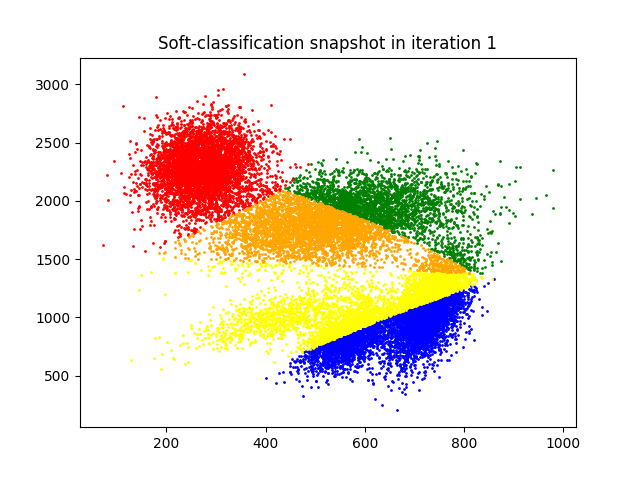
\includegraphics[width=0.6\textwidth]{figures/sc_1.png}
	\caption{Soft-classification snapshot (iteration 1)}
	\label{sc_1}
\end{figure}

\begin{figure}[H]
  \centering
  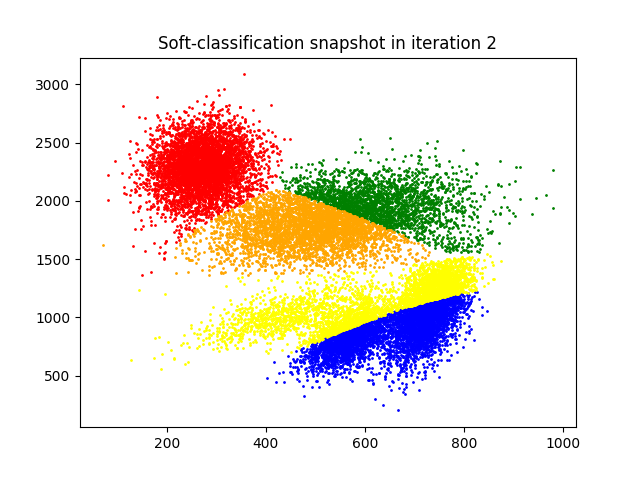
\includegraphics[width=0.6\textwidth]{figures/sc_2.png}
	\caption{Soft-classification snapshot (iteration 2)}
	\label{sc_2}
\end{figure}

\begin{figure}[H]
  \centering
  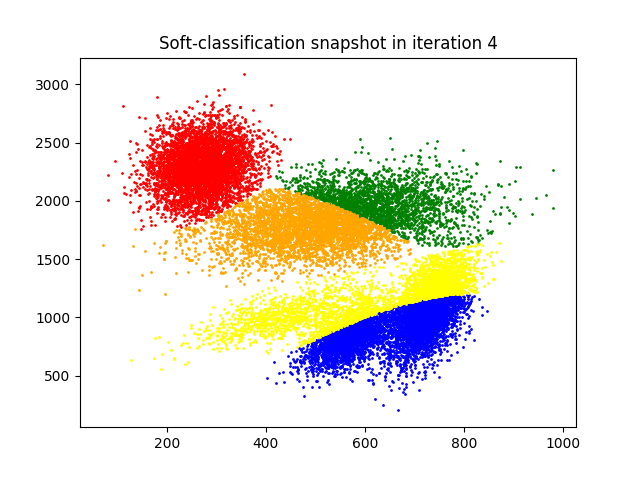
\includegraphics[width=0.6\textwidth]{figures/sc_4.png}
	\caption{Soft-classification snapshot (iteration 4)}
	\label{sc_1}
\end{figure}

\begin{figure}[H]
  \centering
  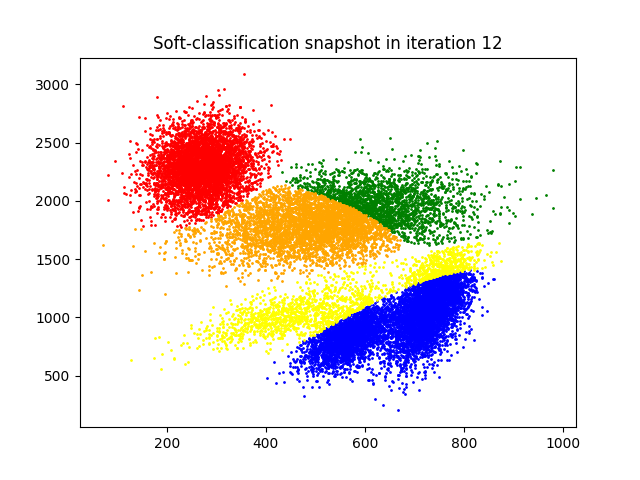
\includegraphics[width=0.6\textwidth]{figures/sc_12.png}
	\caption{Soft-classification snapshot (iteration 12)}
	\label{sc_12}
\end{figure}

\begin{figure}[H]
  \centering
  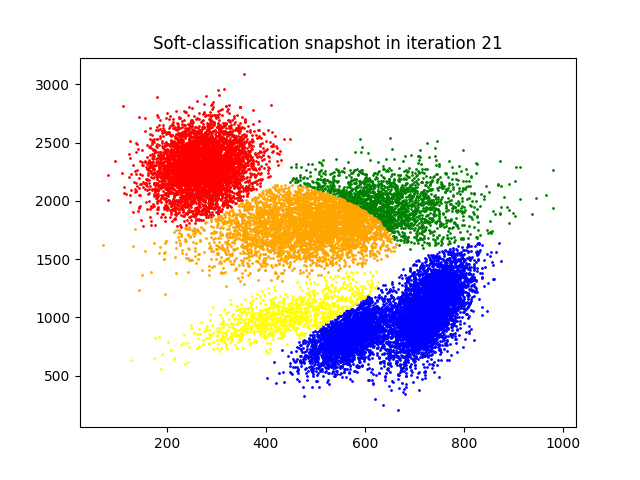
\includegraphics[width=0.6\textwidth]{figures/sc_21.png}
	\caption{Soft-classification snapshot (iteration 21)}
	\label{sc_21}
\end{figure}

\begin{figure}[H]
  \centering
  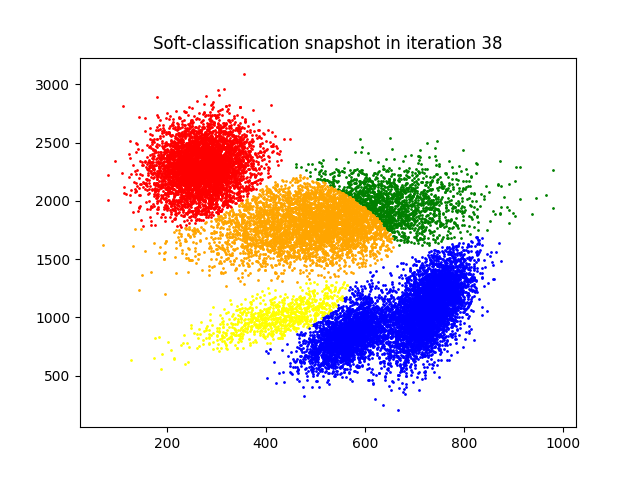
\includegraphics[width=0.6\textwidth]{figures/sc_38.png}
	\caption{Soft-classification snapshot (iteration 38, final)}
	\label{sc_36}
\end{figure}

\textbf{Hint}

Changed random seed gives better classification (more like the one shown in
practical classes). These distributions intiutively match the data better.

\begin{figure}[H]
  \centering
  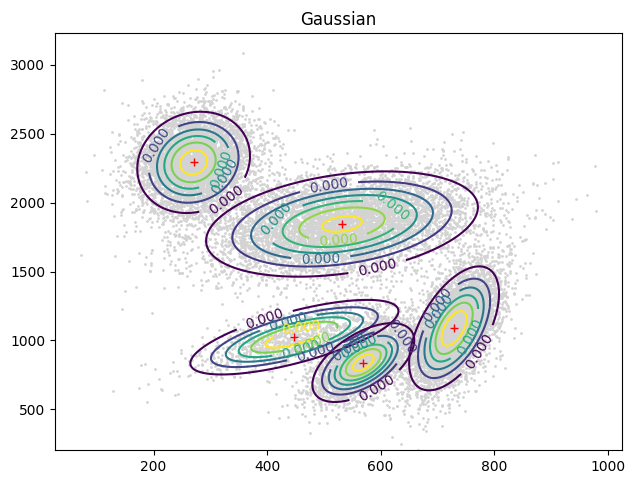
\includegraphics[width=0.8\textwidth]{figures/1_no_seed.png}
	\caption{Better classification with no random seed set}
	\label{1_no_seed}
\end{figure}

\textbf{Findings}

Most important in doing EM would be choosing different starting values for
$\mu_0$ since it cleary effects classification tremendously. Even normalized
values for the data can not prevent this problem. Compared to the test data
fixed random seed from assignement template did not perform well. Different
random starting points for $\mu$ gives high accuracy in some tests.

\end{enumerate}
\newpage
\section{K-means algorithm}

\begin{enumerate}[start=2,label*={\arabic*.}]

  % 2
  \item
  \begin{enumerate}
	  \item Cumulative distance progress $J$ with $\epsilon = 1$

\begin{figure}[H]
  \centering
  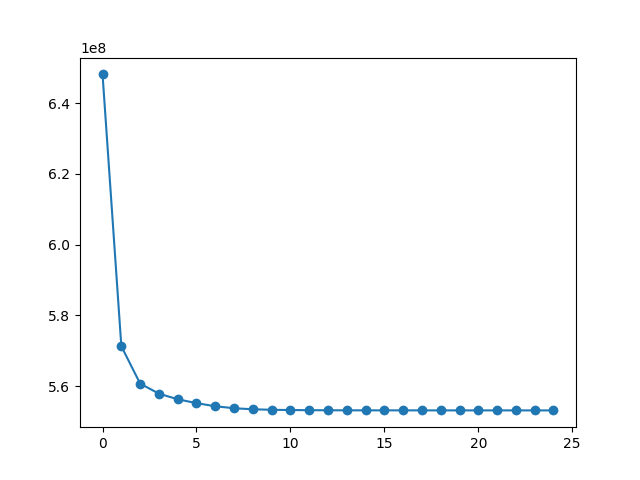
\includegraphics[width=0.8\textwidth]{figures/2_0_distance.png}
	\caption{Distance (cumulative) progress over iterations}
	\label{2_0_distance}
\end{figure}

	  \item Clustering progress
	  
\begin{figure}[H]
  \centering
  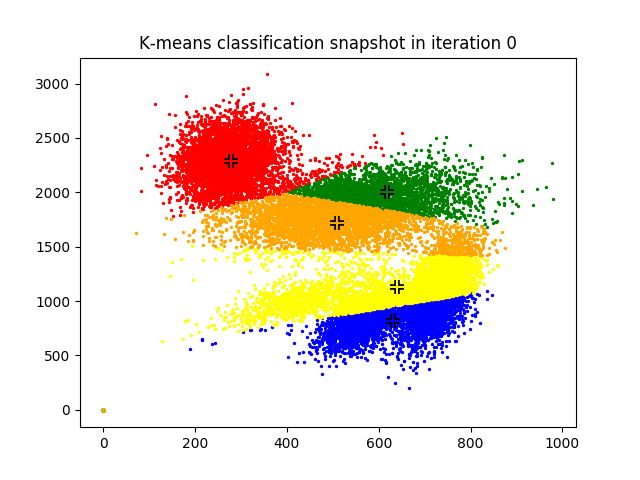
\includegraphics[width=0.6\textwidth]{figures/kmcl_0.png}
	\caption{K-means classification snapshot in iteration 0 (inital)}
	\label{kmcl_0}
\end{figure}

\begin{figure}[H]
  \centering
  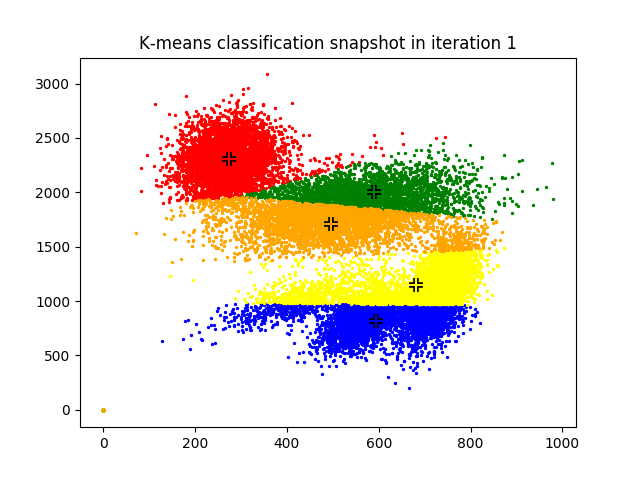
\includegraphics[width=0.6\textwidth]{figures/kmcl_1.png}
	\caption{K-means classification snapshot in iteration 1}
	\label{kmcl_1}
\end{figure}

\begin{figure}[H]
  \centering
  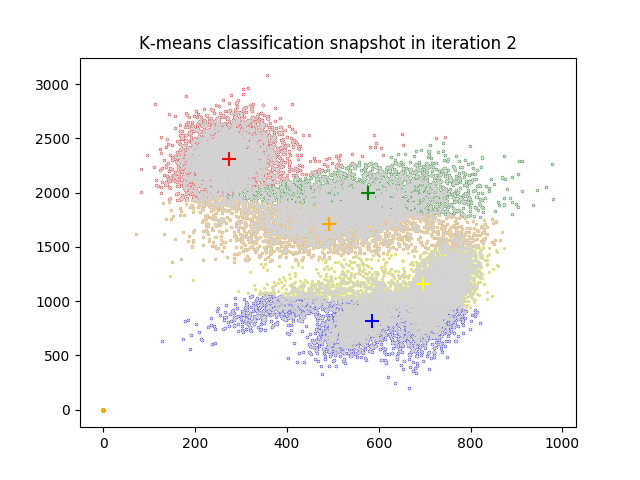
\includegraphics[width=0.6\textwidth]{figures/kmcl_2.png}
	\caption{K-means classification snapshot in iteration 2}
	\label{kmcl_2}
\end{figure}

\begin{figure}[H]
  \centering
  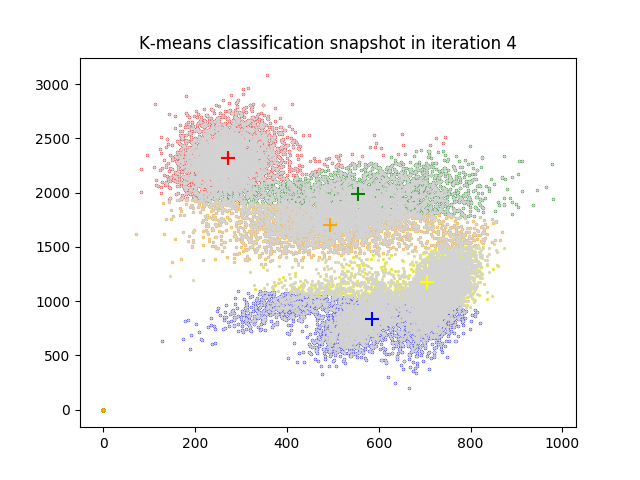
\includegraphics[width=0.6\textwidth]{figures/kmcl_4.png}
	\caption{K-means classification snapshot in iteration 4}
	\label{kmcl_4}
\end{figure}

\begin{figure}[H]
  \centering
  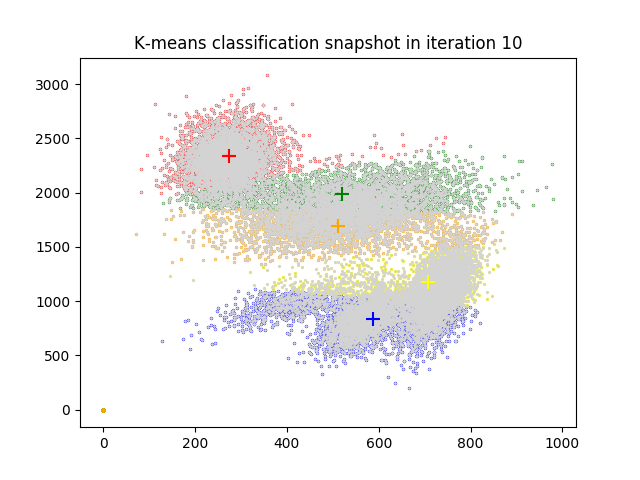
\includegraphics[width=0.6\textwidth]{figures/kmcl_10.png}
	\caption{K-means classification snapshot in iteration 1}
	\label{kmcl_1}
\end{figure}

\begin{figure}[H]
  \centering
  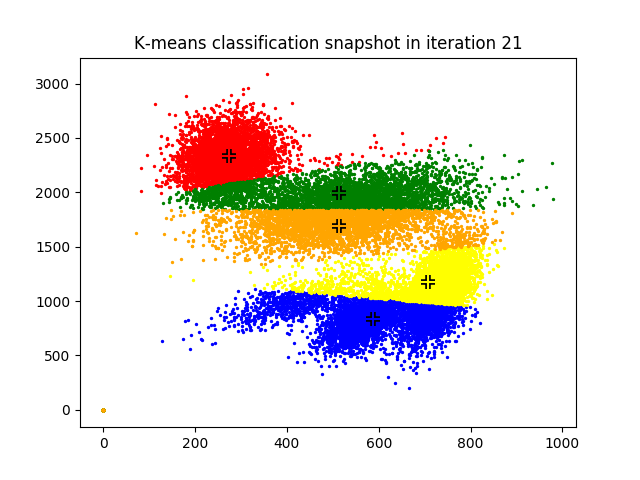
\includegraphics[width=0.6\textwidth]{figures/kmcl_21.png}
	\caption{K-means classification snapshot in iteration 21}
	\label{kmcl_21}
\end{figure}

	  \item Result
	  
\begin{figure}[H]
  \centering
  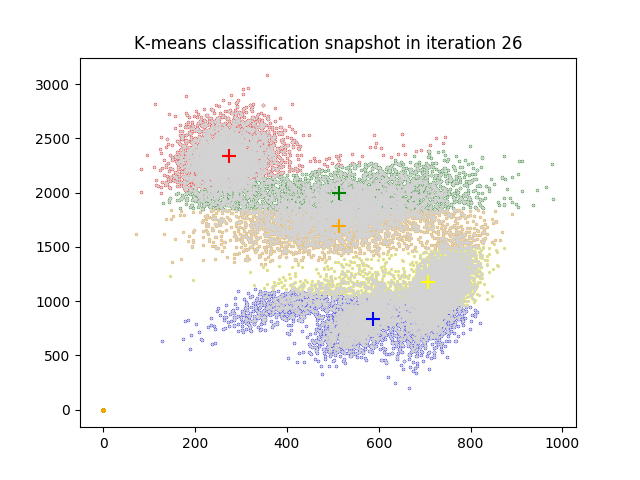
\includegraphics[width=0.6\textwidth]{figures/kmcl_26.png}
	\caption{K-means classification snapshot in iteration 26 (final)}
	\label{kmcl_26}
\end{figure}

  \end{enumerate}
  % 3
  \item Wrong number of compenents

\begin{figure}[H]
  \centering
  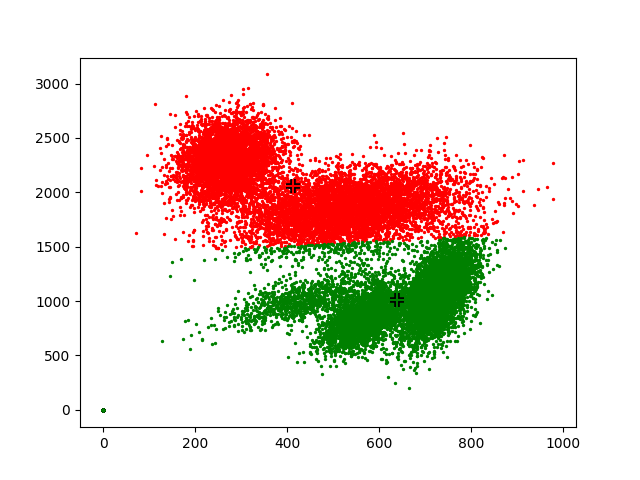
\includegraphics[width=0.6\textwidth]{figures/2_0_m2.png}
	\caption{K-means with wrong number of compenents $m = 2$}
	\label{2_0_m2}
\end{figure}

\begin{figure}[H]
  \centering
  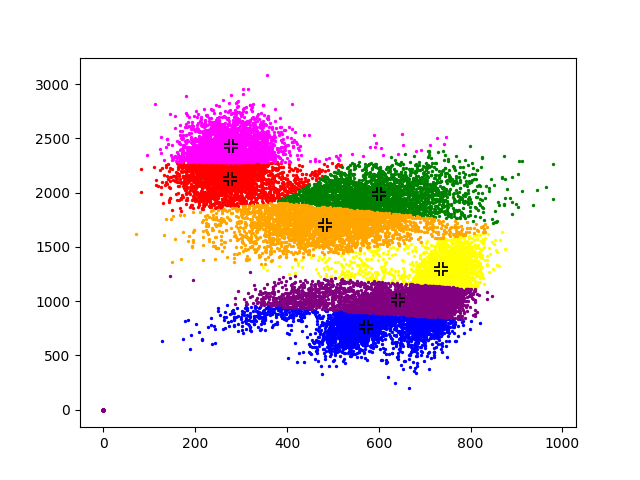
\includegraphics[width=0.6\textwidth]{figures/2_0_m7.png}
	\caption{K-means with wrong number of compenents $m = 7$}
	\label{2_0_m7}
\end{figure}

\textbf{Discussion}

K-means does not perform as good as EM and also has problems with bad start
values for $\mu_0$. The same classes seem to be misclassfied.

\end{enumerate}

\newpage
\section{ Samples from a Gaussian Mixture Model}

\begin{enumerate}[start=1,label*={\arabic*.}]
  % 1
  \item Sampling GMM with $m = 5$, static intial parameters (linear) and 100
  samples.
  
\begin{figure}[H]
  \centering
  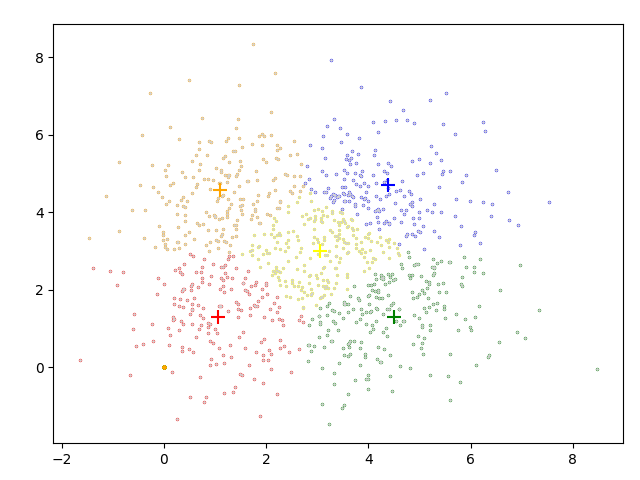
\includegraphics[width=0.6\textwidth]{figures/3_1_km.png}
	\caption{K-means for sampled GMM data $m = 5$}
	\label{3_0_km}
\end{figure} 

\begin{figure}[H]
  \centering
  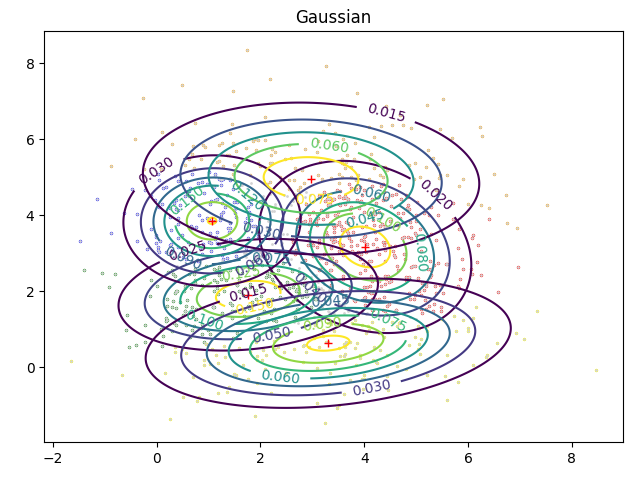
\includegraphics[width=0.6\textwidth]{figures/3_1_EM.png}
	\caption{EM for sampled GMM data $m = 5$}
	\label{3_0_EM}
\end{figure} 

\textbf{Result}

There is still a little TODO in the code for sampling GMM data.

\end{enumerate}

\newpage
\printbibliography

\end{document}